\section{Markov chains}
\label{m:sec:markov}

This section names the process classes used in the thesis and fixes their basic
structure. Methods of analysis are deferred to \cref{m:sec:methods}.

\subsection{Discrete-time Markov chains}
\label{m:sec:dtmc}

A discrete-time Markov chain on a countable state space \(\mathcal S\) is a process
\((X_n)_{n\ge0}\) satisfying
\begin{equation*}
\pr{X_{n+1}=j\mid X_n=i,\,X_{n-1},\dots,X_0}
= \pr{X_{n+1}=j\mid X_n=i}
= P_{ij}.
\end{equation*}
The matrix \(P=(P_{ij})\) is the one-step transition kernel. Absorbing states,
hitting probabilities, and first-step equations are developed as methods in
\cref{m:sec:dt-methods}; the two examples below supply the chains to which those
methods are applied.

\subsubsection{Simple random walks}
\label{m:sec:rw}

\begin{remark}[Scope]
\label{m:rem:rw-todo}
% TODO (Pass~2 stub): expand if user notes or a modelling chapter require more than
% the standard definition below.
What follows is the standard definition for later use; hitting probabilities are
treated as a method in \cref{m:sec:ct-methods}.
\end{remark}

Let \((S_n)_{n\ge0}\) be a simple symmetric random walk on \(\mathbb{Z}\),
\(S_{n+1}=S_n+\xi_{n+1}\) with \(\pr{\xi=\pm1}=\tfrac12\), started at \(S_0=x\).
The one-step transitions are then \(P_{x,x+1}=P_{x,x-1}=\tfrac12\). On a finite
interval with absorbing endpoints (gambler's ruin), first-step analysis
(\cref{m:sec:dt-methods}) yields the classical linear hitting probabilities. Biased
walks and continuous-time analogues reappear as embedded jump chains of birth--death
processes below.

\Cref{m:fig:ruin-hit} records the standard absorbing chain on \(\{0,1,\dots,N\}\)
together with the hitting probabilities \(h_i=\mathbb{P}_i(\tau_N<\tau_0)\) of
reaching the goal \(N\) before ruin at \(0\). For the symmetric walk one has the
linear law \(h_i=i/N\); with upward step probability \(p\neq\tfrac12\) and
\(r=q/p\), \(q=1-p\), the same first-step system gives the curved profile
\(h_i=(r^i-1)/(r^N-1)\).

\begin{figure}[ht]
\centering
\begin{subfigure}[t]{0.96\textwidth}
\centering
\begin{tikzpicture}[
  font=\small,
  state/.style={
    circle, draw=Mblue!75!black, fill=Mblue!10,
    minimum size=0.68cm, inner sep=0pt, thick
  },
  absR/.style={
    circle, draw=Mred!75!black, fill=Mred!12,
    minimum size=0.68cm, inner sep=0pt, thick
  },
  absG/.style={
    circle, draw=Mgreen!60!black, fill=Mgreen!12,
    minimum size=0.68cm, inner sep=0pt, thick
  },
  >=Latex
]
  \node[absR] (n0) at (0,0) {$0$};
  \node[state] (n1) at (1.55,0) {$1$};
  \node[state] (n2) at (3.10,0) {$2$};
  \node[font=\large] (ndots) at (4.45,0) {$\cdots$};
  \node[state] (nNm1) at (5.85,0) {$N{-}1$};
  \node[absG] (nN) at (7.55,0) {$N$};

  % Up arrows from transient states (above)
  \draw[->, thick, Mblue]
    (n1) to[bend left=32] node[above, font=\scriptsize] {$p$} (n2);
  \draw[->, thick, Mblue]
    (n2) to[bend left=32] node[above, font=\scriptsize] {$p$} (ndots);
  \draw[->, thick, Mblue]
    (ndots) to[bend left=32] node[above, font=\scriptsize] {$p$} (nNm1);
  \draw[->, thick, Mblue]
    (nNm1) to[bend left=32] node[above, font=\scriptsize] {$p$} (nN);

  % Down arrows from transient states (below)
  \draw[->, thick, Morange]
    (n1) to[bend left=32] node[below, font=\scriptsize] {$q$} (n0);
  \draw[->, thick, Morange]
    (n2) to[bend left=32] node[below, font=\scriptsize] {$q$} (n1);
  \draw[->, thick, Morange]
    (ndots) to[bend left=32] node[below, font=\scriptsize] {$q$} (n2);
  \draw[->, thick, Morange]
    (nNm1) to[bend left=32] node[below, font=\scriptsize] {$q$} (ndots);

  % Absorbing self-loops
  \draw[->, thick, Mred!70!black]
    (n0) to[out=125,in=55,looseness=6]
    node[above, font=\scriptsize] {$1$} (n0);
  \draw[->, thick, Mgreen!55!black]
    (nN) to[out=125,in=55,looseness=6]
    node[above, font=\scriptsize] {$1$} (nN);

  \node[font=\scriptsize, text=Mred!70!black] at (0,-1.45) {ruin};
  \node[font=\scriptsize, text=Mgreen!50!black] at (7.55,-1.45) {goal};
  \node[font=\scriptsize, text=Mgray] at (3.9,-1.55)
    {symmetric: $p=q=\tfrac12$;\ absorbing at ends};
\end{tikzpicture}
\caption*{(a) Absorbing random walk (gambler's ruin) on $\{0,1,\dots,N\}$.}
\end{subfigure}

\vspace{0.6em}

\begin{subfigure}[t]{0.82\textwidth}
\centering
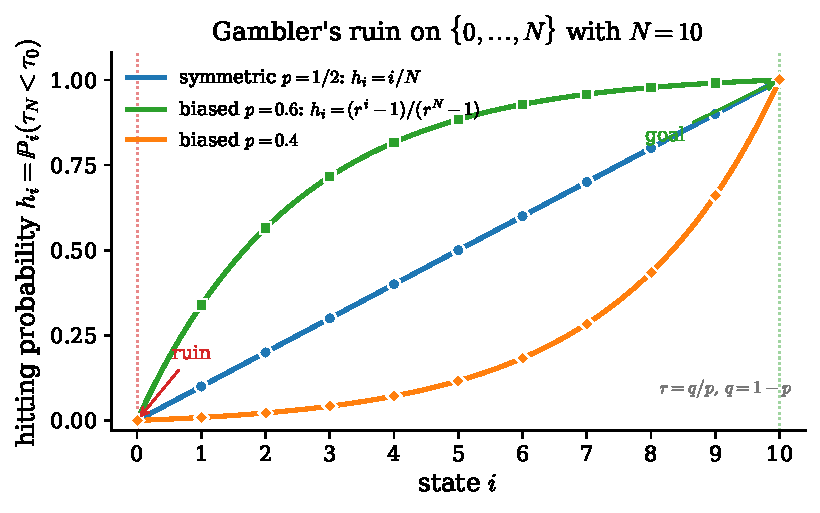
\includegraphics[width=\textwidth]{figures/tikz_gen/ruin_hitting.pdf}
\caption*{(b) Hitting probabilities $h_i=\mathbb{P}_i(\tau_N<\tau_0)$ for $N=10$.}
\end{subfigure}
\caption{Gambler's ruin. Panel~(a): one-step transitions with absorbing endpoints
$0$ (ruin) and $N$ (goal). Panel~(b): probability of hitting $N$ before $0$ from
state $i$, for the symmetric walk $h_i=i/N$ and for biased walks with
$p\in\{0.4,0.6\}$ (where $r=q/p$ and $h_i=(r^i-1)/(r^N-1)$). Markers sit at
integer states; solid curves are the closed-form profiles.}
\label{m:fig:ruin-hit}
\end{figure}

\subsubsection{Galton--Watson processes}
\label{m:sec:gw}

A Galton--Watson process \((Z_n)_{n\ge0}\) is a discrete-time Markov chain on
\(\{0,1,2,\dots\}\) in which each individual independently produces offspring
according to a fixed law, and the next generation is the sum of those contributions.
With offspring probability generating function \(\phi(z)=\ex{z^L}\), the law of
\(Z_n\) is obtained by iterating \(\phi\), and the mean satisfies
\(\ex{Z_n}=m^n\ex{Z_0}\) when \(m=\phi'(1)\).

This thesis uses principally the \emph{binary} (death-or-division) law
\begin{equation}
\label{m:eq:pgfbinary}
\phi(z) = p z^2 + (1-p),
\qquad p\in[0,1],
\end{equation}
for which \(m=2p\) and the survival probability \(S_n=\pr{Z_n>0}\) obeys
\begin{equation}
\label{m:eq:SnIter}
S_{n+1} = 2p\,S_n - p S_n^2,
\qquad S_0=1.
\end{equation}
Extinction is certain for \(p\le\tfrac12\). At criticality \(p=\tfrac12\) one has the
elementary asymptotics \(S_n\sim 2/n\) and infinite expected lifetime; in the
subcritical regime \(p<\tfrac12\) the late-time survival scale involves a constant
\(A(p)\), introduced lightly in \cref{m:sec:condmeans} and developed in full in \ChA.
\Cref{m:fig:gw-binary} summarises the one-step binary law.

\begin{figure}[ht]
\centering
\begin{tikzpicture}[
  font=\small,
  ind/.style={
    circle, draw=Mblue!75!black, fill=Mblue!12,
    minimum size=0.62cm, inner sep=0pt, thick
  },
  dead/.style={
    circle, draw=Mgray, fill=Mgray!12,
    minimum size=0.62cm, inner sep=0pt, thick
  },
  >=Latex
]
  % Parent
  \node[ind] (p) at (0,1.4) {$Z$};
  \node[font=\scriptsize, text=Mgray] at (0,2.05) {generation $n$};

  % Death branch
  \node[dead] (d) at (-2.4,0) {$0$};
  \draw[->, thick, Mred!70!black] (p) -- node[above left, font=\scriptsize] {$1-p$} (d);
  \node[font=\scriptsize, text=Mgray] at (-2.4,-0.55) {death};

  % Division branch
  \node[ind] (a) at (1.6,0) {};
  \node[ind] (b) at (3.0,0) {};
  \draw[->, thick, Mgreen!60!black] (p) -- node[above right, font=\scriptsize, pos=0.45] {$p$} (2.3,0.55);
  \draw[thick, Mgreen!60!black] (2.3,0.55) -- (a);
  \draw[thick, Mgreen!60!black] (2.3,0.55) -- (b);
  \node[font=\scriptsize, text=Mgray] at (2.3,-0.55) {division (two offspring)};

  \node[font=\scriptsize, text=Mgray] at (0.3,-1.2)
    {offspring \pgf{} $\phi(z)=p z^2+(1-p)$,\quad mean $m=2p$};
\end{tikzpicture}
\caption{Binary Galton--Watson step: each individual independently dies (probability
$1-p$) or divides into two (probability $p$). The next generation is the sum of
independent one-step contributions.}
\label{m:fig:gw-binary}
\end{figure}

\begin{remark}[Greater detail later]
\label{m:rem:gw-later}
Critical lifetime theory, the total-progeny (Catalan) law, phase portraits, and the
full quasi-stationary moment calculation for the binary process are deferred:
amplitude theory to \ChA, and modelling-scale applications to later chapters. The
present section keeps only the process class and the one-step structure needed for
\cref{m:sec:methods}.
\end{remark}


\subsection{Continuous-time Markov chains}
\label{m:sec:ctmc-block}

\subsubsection{Exponential clocks}
\label{m:sec:exp}

Every continuous-time model in this thesis is built from events whose rate of occurrence
does not depend on how long the system has already been waiting. That single assumption
forces the exponential distribution.

\begin{definition}[Exponential law]
\label{m:def:exp}
A \rv{} $T$ is exponentially distributed with rate $\theta>0$, written
$T\sim\mathrm{Exp}(\theta)$, if it has density and distribution function
\begin{equation*}
f_T(t) = \theta\ee^{-\theta t},
\qquad
F_T(t) = 1-\ee^{-\theta t},
\qquad t\ge0,
\end{equation*}
and $f_T(t)=0$ for $t<0$. Its mean is $1/\theta$ and its variance $1/\theta^2$.
\end{definition}

The property that matters is memorylessness. For $t_1,t_2>0$,
\begin{equation}
\label{m:eq:memoryless}
\pr{T > t_1+t_2 \mid T > t_1}
= \frac{\ee^{-\theta(t_1+t_2)}}{\ee^{-\theta t_1}}
= \ee^{-\theta t_2}
= \pr{T > t_2},
\end{equation}
so a clock that has already run for time $t_1$ is statistically indistinguishable
from a fresh one. The exponential law is the only continuous distribution with this
property, which is why a process assembled from constant-rate events depends on its
present state alone and not on its history.

When several events compete, the following two facts organise everything that
follows. Let $T_1,\dots,T_m$ be independent with $T_i\sim\mathrm{Exp}(\theta_i)$,
and let $T = \min_i T_i$ be the time of the first event.

\begin{proposition}[Competing clocks]
\label{m:prop:race}
With the notation above, write $\Theta = \sum_{i=1}^m\theta_i$. Then
\begin{equation}
\label{m:eq:race}
T \sim \mathrm{Exp}(\Theta),
\qquad
\pr{T_k = T} = \frac{\theta_k}{\Theta},
\end{equation}
and the identity of the winning clock is independent of $T$.
\end{proposition}

\begin{figure}[ht]
\centering
\begin{tikzpicture}[
  font=\small,
  clock/.style={
    circle, draw=Mblue!80!black, fill=Mblue!12,
    minimum size=1.05cm, inner sep=1pt, thick
  },
  event/.style={
    rounded corners=2pt, draw=Mgray, fill=Mlight,
    minimum width=1.55cm, minimum height=0.55cm, align=center, font=\scriptsize
  },
  >=Latex
]
  % Clocks
  \node[clock] (c1) at (0,0) {$T_1$};
  \node[clock] (c2) at (2.2,0) {$T_2$};
  \node[clock] (c3) at (4.4,0) {$T_3$};
  \node[font=\scriptsize, text=Mgray] at (0,-0.85) {$\mathrm{Exp}(\theta_1)$};
  \node[font=\scriptsize, text=Mgray] at (2.2,-0.85) {$\mathrm{Exp}(\theta_2)$};
  \node[font=\scriptsize, text=Mgray] at (4.4,-0.85) {$\mathrm{Exp}(\theta_3)$};

  % Race arrow
  \draw[->, thick, Mblue] (5.5,0) -- (6.5,0);
  \node[font=\scriptsize, above] at (6.0,0.15) {race};

  % Winner box
  \node[draw=Morange!80!black, fill=Morange!12, thick, rounded corners=3pt,
        minimum width=2.4cm, minimum height=1.6cm, align=center] (win) at (8.2,0)
        {first event\\[2pt]
         $T=\min_i T_i$\\[1pt]
         {\scriptsize $\sim\mathrm{Exp}(\Theta)$}};

  % Bottom: probability of winner
  \node[event] (e1) at (0,-2.1) {event $1$};
  \node[event] (e2) at (2.2,-2.1) {event $2$};
  \node[event] (e3) at (4.4,-2.1) {event $3$};
  \draw[->, Mblue!70] (c1.south) -- (e1.north);
  \draw[->, Mblue!70] (c2.south) -- (e2.north);
  \draw[->, Mblue!70] (c3.south) -- (e3.north);
  \node[font=\scriptsize, text=Mgray] at (2.2,-2.85)
    {$\displaystyle\pr{T_k=T}=\frac{\theta_k}{\Theta},\quad
      \Theta=\sum_i\theta_i$};
\end{tikzpicture}
\caption{Competing exponential clocks (\cref{m:prop:race}): independent holding times
race; the minimum is exponential with rate $\Theta$, and the winning event is chosen
with probability proportional to its rate, independently of the waiting time.}
\label{m:fig:competing-clocks}
\end{figure}

\begin{proof}
For the first claim,
$\pr{T>t} = \prod_i\pr{T_i>t} = \prod_i\ee^{-\theta_i t} = \ee^{-\Theta t}$.
For the second, condition on the value of $T_k$ and use independence:
\begin{equation*}
\pr{T_k = T}
= \int_0^\infty \theta_k\ee^{-\theta_k u}\prod_{i\neq k}\ee^{-\theta_i u}\,\dd u
= \theta_k\int_0^\infty \ee^{-\Theta u}\,\dd u
= \frac{\theta_k}{\Theta}.
\end{equation*}
Repeating the calculation with the integral truncated at $t$ gives
$\pr{T_k=T,\ T>t} = (\theta_k/\Theta)\ee^{-\Theta t}
= \pr{T_k=T}\pr{T>t}$, which is the asserted independence.
\end{proof}

\Cref{m:prop:race} is used in two ways. First, a rate $\theta_k$ becomes a
probability $\theta_k/\Theta$ as soon as one asks which of several things happened
rather than when; \cref{m:sec:cts} uses exactly this to identify the replication
probability $p$ of a discrete-generation model with $\lambda/(\lambda+\mu)$ in a
continuous-time one. Second, the same proposition is the entire content of the
direct simulation method.

\begin{remark}[Direct simulation]
\label{m:rem:gillespie}
\Cref{m:prop:race} is an algorithm as well as a theorem. Given the current state,
compute the rate $\theta_i$ of every possible event and their sum $\Theta$; draw
$T\sim\mathrm{Exp}(\Theta)$ by inverting the distribution function of
\cref{m:def:exp} on a uniform variate; draw the event $k$ with probability
$\theta_k/\Theta$; advance the clock by $T$, apply event $k$, and repeat. Because
the two draws are independent and the exponential law is memoryless, the resulting
trajectory has exactly the law of the process. This is Gillespie's direct method
\cite{Gillespie1977}; in this thesis it is used to check analytical results, never to
replace them.
\end{remark}



\subsubsection{Generators and master equations}
\label{m:sec:ctmc}

Let $\{X_t : t\ge0\}$ be a stochastic process taking values in a countable state
space $\mathcal S$, which throughout will be a set of population counts or of
tuples of counts. The process is a \emph{continuous-time Markov chain} if, for all
times $s,t\ge0$ and all states,
\begin{equation}
\label{m:eq:markov}
\pr{X_{t+s} = j \mid X_t = i,\ \{X_u\}_{u<t}} = \pr{X_{t+s}=j\mid X_t = i},
\end{equation}
so that the past influences the future only through the present. The chain is
\emph{time homogeneous} if the right-hand side depends on $s$ but not on $t$, in
which case one writes $p_{ij}(s) = \pr{X_{t+s}=j\mid X_t=i}$. All chains in this thesis are time homogeneous unless stated otherwise; the
time-inhomogeneous case is outlined in \cref{m:sec:time-inhom}.

Such a chain is specified by its \emph{generator}, the matrix $Q = (q_{ij})$ whose
off-diagonal entries are the rates of the corresponding transitions,
\begin{equation}
\label{m:eq:generator}
q_{ij} = \lim_{\Delta t\to0}\frac{p_{ij}(\Delta t)}{\Delta t}\quad(j\neq i),
\qquad
q_{ii} = -\sum_{j\neq i}q_{ij} =: -q_i ,
\end{equation}
so that every row of $Q$ sums to zero. Equivalently, and this is the form used to
define models below,
\begin{equation}
\label{m:eq:infinitesimal}
\pr{X_{t+\Delta t} = j \mid X_t = i} = q_{ij}\,\Delta t + o(\Delta t)
\qquad (j \neq i),
\end{equation}
with the complementary probability $1-q_i\Delta t + o(\Delta t)$ of no transition
at all. By \cref{m:prop:race} the chain leaves state $i$ after a holding time
distributed as $\mathrm{Exp}(q_i)$ and then jumps to $j$ with probability
$q_{ij}/q_i$. A state with $q_i=0$ is \emph{absorbing}: the chain that reaches it
stays there forever. Extinction and rupture will both be modelled as absorbing
states, and the whole of \cref{m:sec:condmeans} concerns the behaviour of a chain
conditioned on not yet having been absorbed.

Differentiating the Chapman--Kolmogorov identity
$p_{ij}(t+\Delta t) = \sum_k p_{ik}(t)p_{kj}(\Delta t)$ with respect to $\Delta t$
at $\Delta t=0$ gives the \emph{forward Kolmogorov equations},
\begin{equation}
\label{m:eq:kolmogorov}
\ddt{p_{ij}(t)} = \sum_{k} p_{ik}(t)\,q_{kj},
\qquad\text{that is}\qquad
\dda{P}{t} = P\,Q .
\end{equation}
Written out for a fixed initial state and with $p_j(t)$ for the probability of
occupying state $j$ at time $t$, \cref{m:eq:kolmogorov} becomes the master equation
\begin{equation}
\label{m:eq:master}
\ddt{p_j(t)} = \sum_{k\neq j}q_{kj}\,p_k(t) - q_j\,p_j(t):
\end{equation}
probability flows into state $j$ from every state that can reach it and out of $j$
at total rate $q_j$. Every model in this thesis is specified by writing down
\cref{m:eq:infinitesimal} and then reading off \cref{m:eq:master}.


\subsubsection{Probability generating functions}
\label{m:sec:pgf}

For a \rv{} $X$ taking values in $\{0,1,2,\dots\}$ with $p_k = \pr{X=k}$, the
\pgf{} is
\begin{equation}
\label{m:eq:pgfdef}
\phi(z) = \ex{z^X} = \sum_{k=0}^{\infty}p_k z^k ,
\end{equation}
which converges at least for $|z|\le1$ since the $p_k$ sum to one. The series
determines the distribution --- $p_k = \phi^{(k)}(0)/k!$ --- and moments are read
off at $z=1$:
\begin{equation}
\label{m:eq:pgfmoments}
\phi(1) = 1,
\qquad
\phi'(1) = \ex{X},
\qquad
\phi''(1) = \ex{X(X-1)} .
\end{equation}
Two structural properties do most of the work. If $X$ and $Y$ are independent then
$\phi_{X+Y} = \phi_X\phi_Y$, so sums become products. And if $N$ is an independent
count with \pgf{} $\psi$, the random sum $X_1+\dots+X_N$ of independent copies of
$X$ has \pgf{} $\psi\circ\phi$; composition of generating functions is what makes
branching processes tractable, and \cref{m:sec:gw} rests on it.

For a pair of counts the definition extends to
\begin{equation}
\label{m:eq:pgfbivariate}
G(x,y) = \ex{x^{X}y^{Y}} = \sum_{i}\sum_{j}\pr{X=i,\,Y=j}\,x^iy^j ,
\end{equation}
with marginals recovered by setting the other variable to one. The absorption
models of \cref{m:sec:moc} track particles inside and outside a compartment and
therefore need this bivariate form; \cref{m:app:extract} records how to invert it.

When the counts evolve in time, $G$ acquires a time argument,
$G(x,y,t) = \ex{x^{X_t}y^{Y_t}}$, and the master equation \cref{m:eq:master} for the
infinite family of state probabilities collapses to a single partial differential
equation for $G$. The mechanism is uniform: multiply the equation for
$p_{ij}(t)$ by $x^iy^j$, sum over all states, shift indices so that every sum is
again of the form \cref{m:eq:pgfbivariate}, and recognise the factors of $i$ and $j$
produced by the linear rates as derivatives $\partial_x$ and $\partial_y$. Because
the rates in these models are linear in the counts, the resulting equation is
always of first order, and the method of characteristics therefore always applies
in principle. \Cref{m:sec:linbd} carries this out in the simplest case;
\cref{m:sec:moc} does it three times over.


\subsubsection{Poisson processes}
\label{m:sec:poisson}

\begin{remark}[Scope]
\label{m:rem:poisson-todo}
% TODO (Pass~2 stub): expand if a later chapter needs a fuller Poisson development.
The paragraph below records the standard link between Poisson processes, exponential
clocks, and pure birth.
\end{remark}

A homogeneous Poisson process \((N_t)_{t\ge0}\) of rate \(\theta>0\) is the counting
process with independent increments and \(N_t\sim\mathrm{Poisson}(\theta t)\).
Equivalently, the inter-event times are i.i.d.\ \(\mathrm{Exp}(\theta)\). A pure-birth
process with constant per-capita birth rate is a Yule process; with a single individual
and no death it reduces to a Poisson process of events. Competing exponential clocks
(\cref{m:prop:race}) build general continuous-time Markov chains from the same
holding-time law. \Cref{m:fig:poisson-path} shows one sample counting path together
with the exponential interarrival density that generates it; the mean line
\(\ex{N_t}=\theta t\) provides the deterministic scale against which the jumps
fluctuate.

\begin{figure}[ht]
\centering
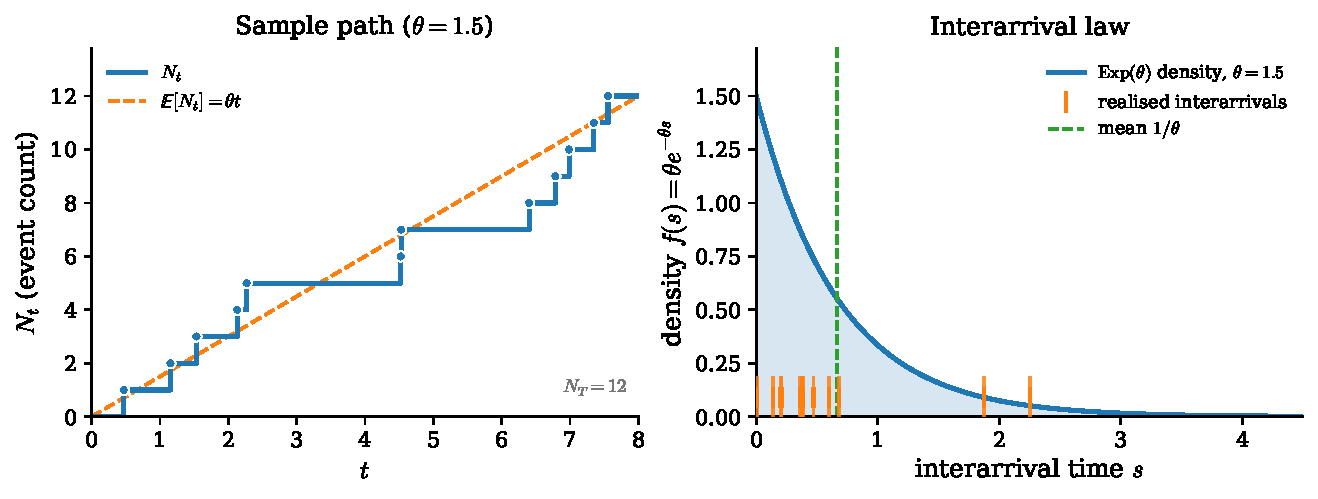
\includegraphics[width=0.94\textwidth]{figures/tikz_gen/poisson_path.pdf}
\caption{Homogeneous Poisson process of rate $\theta=1.5$. Left: a sample path of the
counting process $N_t$ (step function) with event markers, and the mean trajectory
$\ex{N_t}=\theta t$ (dashed). Right: density $f(s)=\theta\ee^{-\theta s}$ of the
i.i.d.\ $\mathrm{Exp}(\theta)$ interarrival times, with the realised waits from the
left-hand path marked as a rug and the mean wait $1/\theta$ indicated.}
\label{m:fig:poisson-path}
\end{figure}

\subsubsection{Birth--death processes}
\label{m:sec:linbd}

The linear birth--death process is the continuous-time counterpart of the
Galton--Watson process, and it is the last piece of standard machinery needed.
Let $X_t$ count individuals, each of which independently gives birth at rate
$\lambda$ and dies at rate $\mu$. In the notation of \cref{m:eq:infinitesimal} the
non-zero rates out of state $n$ are
\begin{equation}
\label{m:eq:bdrates}
q_{n,n+1} = \lambda n,
\qquad
q_{n,n-1} = \mu n ,
\end{equation}
so that $q_n = (\lambda+\mu)n$ and $n=0$ is absorbing; see the rate diagram in
\cref{m:fig:bd-chain}. The master equation
\cref{m:eq:master} reads
\begin{equation}
\label{m:eq:bdmaster}
\ddt{p_n(t)} = \lambda(n-1)p_{n-1}(t) + \mu(n+1)p_{n+1}(t) - (\lambda+\mu)n\,p_n(t).
\end{equation}

\begin{figure}[ht]
\centering
\begin{tikzpicture}[
  font=\small,
  state/.style={
    circle, draw=Mblue!75!black, fill=Mblue!10,
    minimum size=0.78cm, inner sep=0pt, thick
  },
  abs/.style={
    circle, draw=Mred!75!black, fill=Mred!10,
    minimum size=0.78cm, inner sep=0pt, thick
  },
  >=Latex
]
  \node[abs] (n0) at (0,0) {$0$};
  \node[state] (n1) at (2.0,0) {$1$};
  \node[state] (n2) at (4.0,0) {$2$};
  \node[state] (n3) at (6.0,0) {$3$};
  \node[font=\large] (ndots) at (7.6,0) {$\cdots$};

  % Birth arrows (above)
  \draw[->, thick, Mgreen!70!black]
    (n1) to[bend left=28] node[above, font=\scriptsize] {$\lambda$} (n2);
  \draw[->, thick, Mgreen!70!black]
    (n2) to[bend left=28] node[above, font=\scriptsize] {$2\lambda$} (n3);
  \draw[->, thick, Mgreen!70!black]
    (n3) to[bend left=28] node[above, font=\scriptsize] {$3\lambda$} (ndots);

  % Death arrows (below)
  \draw[->, thick, Mred!70!black]
    (n1) to[bend left=28] node[below, font=\scriptsize] {$\mu$} (n0);
  \draw[->, thick, Mred!70!black]
    (n2) to[bend left=28] node[below, font=\scriptsize] {$2\mu$} (n1);
  \draw[->, thick, Mred!70!black]
    (n3) to[bend left=28] node[below, font=\scriptsize] {$3\mu$} (n2);
  \draw[->, thick, Mred!70!black]
    (ndots) to[bend left=28] node[below, font=\scriptsize] {} (n3);

  % Legend
  \node[font=\scriptsize, text=Mgreen!50!black] at (1.0,1.35) {birth};
  \node[font=\scriptsize, text=Mred!60!black] at (1.0,-1.35) {death};
  \node[font=\scriptsize, text=Mgray, align=left] at (9.3,0)
    {absorbing\\[1pt]$n=0$};
  \draw[->, Mgray, thin] (8.6,-0.15) -- (n0.east);
\end{tikzpicture}
\caption{Linear birth--death process on $\{0,1,2,\dots\}$: per-capita rates
$\lambda$ (birth) and $\mu$ (death) yield transition rates $q_{n,n+1}=\lambda n$
and $q_{n,n-1}=\mu n$. State $0$ is absorbing (extinction).}
\label{m:fig:bd-chain}
\end{figure}
Multiplying by $z^n$ and summing over $n\ge0$, the three terms become
$\lambda z^2\partial_zG$, $\mu\,\partial_zG$ and $-(\lambda+\mu)z\,\partial_zG$
after the index shifts described above, so that
\begin{equation}
\label{m:eq:bdpde}
\pddt{G} = \bigl(\lambda z^2 - (\lambda+\mu)z + \mu\bigr)\pdd{G}{z}
= (\lambda z-\mu)(z-1)\pdd{G}{z},
\qquad G(z,0) = z^{N},
\end{equation}
for a process started from $N$ individuals. The quadratic coefficient factorises
with roots $z=1$ and $z=\mu/\lambda$; the same factorisation, in a different
variable, reappears in \cref{m:sec:absbirthdeath} and is what makes that calculation
possible. Solving \cref{m:eq:bdpde} along its characteristics gives the classical
result of Kendall \cite{Kendall1948},
\begin{equation}
\label{m:eq:bdsolution}
G(z,t) = \lrb{\frac{\mu(1-z) - (\mu-\lambda z)\ee^{-(\lambda-\mu)t}}
{\lambda(1-z) - (\mu-\lambda z)\ee^{-(\lambda-\mu)t}}}^{\!N},
\qquad \lambda\neq\mu .
\end{equation}
Two consequences are needed later. The mean follows from
\cref{m:eq:pgfmoments} or, more quickly, from the fact that each individual
contributes independently:
\begin{equation}
\label{m:eq:bdmean}
\ex{X_t} = N\ee^{(\lambda-\mu)t}.
\end{equation}
The probability of extinction by time $t$ is $p_0(t) = G(0,t)$, that is
\begin{equation}
\label{m:eq:p0t}
p_0(t) =
\begin{cases}
\displaystyle\lrb{\frac{\mu-\mu\ee^{(\mu-\lambda)t}}{\lambda-\mu\ee^{(\mu-\lambda)t}}}^{\!N},
& \lambda\neq\mu,\\[14pt]
\displaystyle\lrb{\frac{\lambda t}{1+\lambda t}}^{\!N},
& \lambda=\mu,
\end{cases}
\end{equation}
the critical case following by taking $\mu\to\lambda$ in the first line. Letting
$t\to\infty$ recovers the familiar threshold: extinction is certain when
$\lambda\le\mu$, and occurs with probability $(\mu/\lambda)^N$ when
$\lambda>\mu$. \Cref{m:fig:bd-curves} plots the mean and survival curves in the
three regimes; \cref{m:sec:cts} takes \cref{m:eq:p0t} as its starting point.

\begin{figure}[ht]
\centering
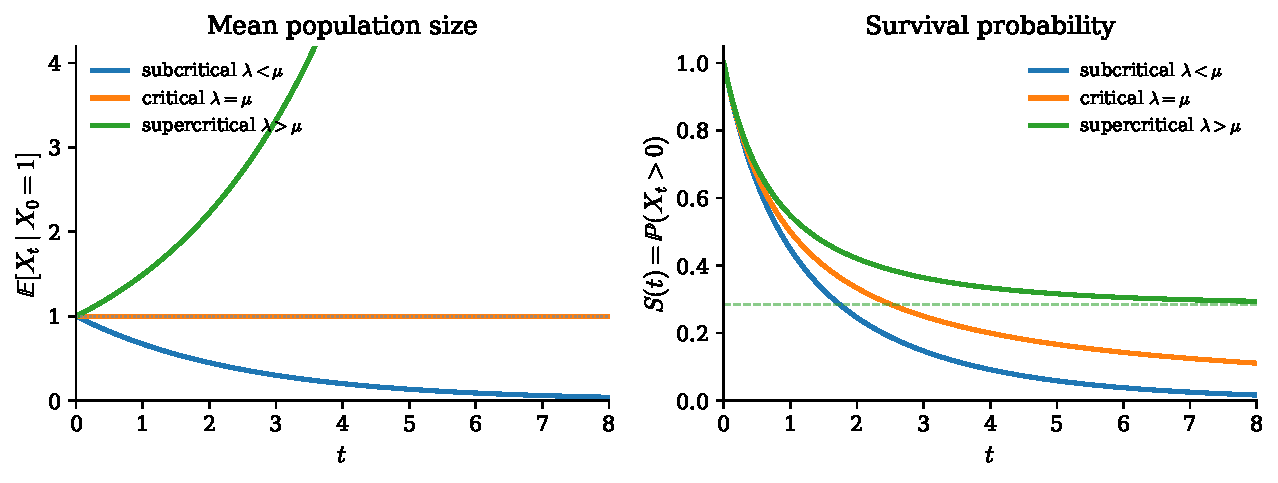
\includegraphics[width=0.92\textwidth]{figures/tikz_gen/bd_mean_survival_panel.pdf}
\caption{Linear birth--death process started from one individual: mean population
size (left) and survival probability $S(t)=\pr{X_t>0}$ (right) for subcritical
($\lambda=0.6$, $\mu=1$), critical ($\lambda=\mu=1$), and supercritical
($\lambda=1.4$, $\mu=1$) rates. In the supercritical case the survival probability
approaches $1-\mu/\lambda$ (dashed).}
\label{m:fig:bd-curves}
\end{figure}

\subsubsection{Birth--death--catastrophe processes}
\label{m:sec:ctbdc}

The discrete rupture mechanism of earlier drafts has a continuous-time counterpart,
and since that process is the central object of several later chapters it is defined
here in the notation already fixed. No results about it are derived in this chapter.

\begin{definition}[Birth--death--catastrophe process]
\label{m:def:bdc}
Let $X_t$ count individuals in a compartment. Each individual independently gives
birth at rate $\lambda$ and dies at rate $\mu$, and the compartment additionally
undergoes a catastrophe --- a rupture that removes the entire population at once
--- at a rate $\rho$ per individual, so that the total catastrophe rate in state
$n$ is $\rho n$. Writing $\dagger$ for the post-catastrophe state, the non-zero
transition rates out of $n\ge1$ are
\begin{equation}
\label{m:eq:bdcrates}
q_{n,n+1} = \lambda n,
\qquad
q_{n,n-1} = \mu n,
\qquad
q_{n,\dagger} = \rho n ,
\end{equation}
and both $n=0$ and $\dagger$ are absorbing (\cref{m:fig:bdc-chain}).
\end{definition}

\begin{figure}[ht]
\centering
\begin{tikzpicture}[
  font=\small,
  state/.style={
    circle, draw=Mblue!75!black, fill=Mblue!10,
    minimum size=0.72cm, inner sep=0pt, thick
  },
  abs/.style={
    circle, draw=Mred!75!black, fill=Mred!10,
    minimum size=0.72cm, inner sep=0pt, thick
  },
  cat/.style={
    circle, draw=Mpurple!80!black, fill=Mpurple!12,
    minimum size=0.82cm, inner sep=0pt, thick
  },
  >=Latex
]
  \node[abs] (n0) at (0,0) {$0$};
  \node[state] (n1) at (2.0,0) {$1$};
  \node[state] (n2) at (4.0,0) {$2$};
  \node[state] (n3) at (6.0,0) {$3$};
  \node[font=\large] (ndots) at (7.55,0) {$\cdots$};
  \node[cat] (dag) at (4.0,-2.15) {$\dagger$};

  % Birth
  \draw[->, thick, Mgreen!70!black]
    (n1) to[bend left=26] node[above, font=\scriptsize] {$\lambda$} (n2);
  \draw[->, thick, Mgreen!70!black]
    (n2) to[bend left=26] node[above, font=\scriptsize] {$2\lambda$} (n3);
  \draw[->, thick, Mgreen!70!black]
    (n3) to[bend left=26] node[above, font=\scriptsize] {$3\lambda$} (ndots);

  % Death
  \draw[->, thick, Mred!70!black]
    (n1) to[bend left=26] node[below, font=\scriptsize, pos=0.45] {$\mu$} (n0);
  \draw[->, thick, Mred!70!black]
    (n2) to[bend left=26] node[below, font=\scriptsize, pos=0.45] {$2\mu$} (n1);
  \draw[->, thick, Mred!70!black]
    (n3) to[bend left=26] node[below, font=\scriptsize, pos=0.45] {$3\mu$} (n2);

  % Catastrophe (to dagger)
  \draw[->, thick, Mpurple!80!black]
    (n1.south) to[out=-70,in=160] node[left, font=\scriptsize, pos=0.45] {$\rho$} (dag.west);
  \draw[->, thick, Mpurple!80!black]
    (n2.south) -- node[right, font=\scriptsize, pos=0.4] {$2\rho$} (dag.north);
  \draw[->, thick, Mpurple!80!black]
    (n3.south) to[out=-110,in=20] node[right, font=\scriptsize, pos=0.45] {$3\rho$} (dag.east);

  % Labels
  \node[font=\scriptsize, text=Mred!60!black, align=center] at (-0.15,0.95)
    {extinction\\absorbing};
  \node[font=\scriptsize, text=Mpurple!70!black, align=center] at (6.5,-2.15)
    {catastrophe\\absorbing};
\end{tikzpicture}
\caption{Birth--death--catastrophe process: the birth--death chain on the positive
integers is killed at per-capita rate $\rho$, sending the process to a second
absorbing state $\dagger$ (catastrophe/rupture). Extinction ($0$) and catastrophe
($\dagger$) are distinct absorbing mechanisms.}
\label{m:fig:bdc-chain}
\end{figure}

Two features distinguish \cref{m:def:bdc} from the linear birth--death process of
\cref{m:sec:linbd}, and both matter later. The process now has \emph{two} absorbing
states, reached by mechanisms that are distinguishable and not interchangeable:
extinction empties the compartment gradually, catastrophe empties it in one event
and releases its contents. And the catastrophe rate is proportional to the
population, so the compartment becomes more likely to rupture the fuller it is.

The generating-function machinery of \cref{m:sec:pgf} applies unchanged. Restricting
attention to realisations that have not yet ruptured and writing
$G(z,t) = \ex{z^{X_t}\mathbf 1\{X_t\neq\dagger\}}$, the master equation for
\cref{m:eq:bdcrates} yields
\begin{equation}
\label{m:eq:bdcpde}
\pddt{G} = \bigl(\lambda z^2-(\lambda+\mu+\rho)z+\mu\bigr)\pdd{G}{z},
\qquad G(z,0) = z^{N},
\end{equation}
which differs from \cref{m:eq:bdpde} only in the coefficient of $z$. The quadratic no
longer factorises with a root at $z=1$, and that single change is responsible for
most of what is interesting about the process: probability is not conserved on the
non-ruptured states, and $G(1,t)$ is the survival probability rather than one.
Rates, means and variances, state probabilities and the associated
generating-function equations are developed \fwd{bdc}{in the later chapters on
birth--death--catastrophe processes}, with the two-type extension treated
\fwd{multitype}{in the chapter on multi-type processes} and the release of a
ruptured compartment's contents into a shared medium
\fwd{rupture}{in the chapter on compartment rupture}. The method used to solve
\cref{m:eq:bdcpde} and its relatives is the subject of \cref{m:sec:moc}.



\subsubsection*{Discrete rupture as a killed chain}
\label{m:sec:killed-bdc}

The continuous-time process of \cref{m:def:bdc} may also be viewed as a birth--death
process killed at a state-dependent rate. Restricting the generator to the positive
states produces a killed subgenerator $Q^\dagger$ whose off-diagonal entries are the
birth and death rates and whose diagonal absorbs the catastrophe rate $\rho n$. A
quasi-stationary distribution $\nu$ on $\{1,2,\dots\}$, when it exists, satisfies
the left eigenrelation
\begin{equation}
\label{m:eq:bdc-qsd-eigenrelation}
\nu Q^\dagger = -\gamma\,\nu,
\qquad \nu\mathbf 1=1,
\end{equation}
for some decay parameter $\gamma>0$: under $\nu$, the residual lifetime to absorption
(by death or by catastrophe) is exponential with rate $\gamma$, and the conditional
law of the population given non-absorption is stationary. The present chapter needs
only the distinction between the two absorbing mechanisms and the form of
\cref{m:eq:bdc-qsd-eigenrelation}; rates, means and the full spectral theory belong
to later modelling chapters.

\begin{remark}[Catastrophe is not a mean-field hazard]
\label{m:rem:catastrophe-not-meanfield}
A catastrophe rate proportional to population size is a genuine jump mechanism on
the state space, not a deterministic hazard applied to the mean trajectory. Replacing
the random census $Z_i$ by $\ex{Z_i}$ in discrete survival formulae such as
replacing the random census by its mean systematically understates survival (Jensen), and confuses
non-rupture with non-extinction. The two events are distinct, and joint
conditioning on neither is a separate problem.
\end{remark}


\subsection{Time-inhomogeneous processes}
\label{m:sec:time-inhom}

\subsubsection{Logistic speciation model}
\label{m:sec:logistic-speciation}

\begin{remark}[TODO --- logistic speciation]
\label{m:rem:logistic-todo}
No logistic speciation (time-inhomogeneous) model is developed in this chapter yet.
Intended content, pending notes or references: a continuous-time process whose birth
or death rates depend explicitly on absolute time (or on a deterministic environmental
schedule), with logistic density dependence in the speciation or birth rate; the
generator form; contrast with the time-homogeneous birth--death process of
\cref{m:sec:linbd}; and a pointer to any later chapter that uses the model.
\end{remark}

\subsection{Coupled ODE--CTMC systems}
\label{m:sec:coupled}

\begin{remark}[TODO --- concrete coupling examples]
\label{m:rem:coupled-todo}
% TODO (Pass~2 stub): import a concrete thesis model when notes are available.
The framework below is abstract; concrete examples are deferred to the modelling
chapters that use them.
\end{remark}

Several models in the wider thesis couple a continuous-time Markov chain \((X_t)\) on
a discrete state space to an ordinary differential equation for a continuous state
\(y_t\in\mathbb{R}^d\). Three dependence patterns arise.

\begin{enumerate}[label=\textup{(\roman*)}]
\item \emph{ODE driven by the chain:} \(\dot y = f(y,X_t)\), so the vector field
jumps when the chain jumps, while the chain's rates may be constant or depend only
on \(X\).
\item \emph{Chain driven by the ODE:} the transition rates \(q_{ij}(y_t)\) of the
chain depend on the continuous state, while \(\dot y = f(y)\) evolves autonomously
between jumps (or continuously).
\item \emph{Two-way coupling:} both \(f=f(y,X)\) and \(q_{ij}=q_{ij}(y)\) are
active, so neither component is autonomous.
\end{enumerate}

Piecewise-deterministic Markov processes formalise (i)--(iii) when the continuous
motion is deterministic between jumps (\cref{m:fig:coupled-schematic}). The
exponential-clock construction of \cref{m:sec:exp} still supplies the holding times
once rates are frozen at the current \((y,X)\); between jumps one integrates the ODE.

\begin{figure}[ht]
\centering
\begin{tikzpicture}[
  font=\small,
  box/.style={
    draw=Mblue!70!black, fill=Mblue!8, thick, rounded corners=3pt,
    minimum width=2.35cm, minimum height=1.05cm, align=center
  },
  chainbox/.style={
    draw=Morange!75!black, fill=Morange!10, thick, rounded corners=3pt,
    minimum width=2.35cm, minimum height=1.05cm, align=center
  },
  >=Latex
]
  % (i)
  \begin{scope}[shift={(0,0)}]
    \node[font=\bfseries\scriptsize, text=Mgray] at (1.2,2.0) {(i) ODE driven by chain};
    \node[chainbox] (Xi) at (1.2,1.15) {$X_t$\\{\scriptsize CTMC}};
    \node[box] (yi) at (1.2,0) {$y_t$\\{\scriptsize ODE}};
    \draw[->, thick, Mblue] (Xi) -- node[right, font=\scriptsize] {$f(y,X)$} (yi);
  \end{scope}

  % (ii)
  \begin{scope}[shift={(4.6,0)}]
    \node[font=\bfseries\scriptsize, text=Mgray] at (1.2,2.0) {(ii) chain driven by ODE};
    \node[chainbox] (Xii) at (1.2,1.15) {$X_t$\\{\scriptsize CTMC}};
    \node[box] (yii) at (1.2,0) {$y_t$\\{\scriptsize ODE}};
    \draw[->, thick, Morange] (yii) -- node[right, font=\scriptsize] {$q_{ij}(y)$} (Xii);
  \end{scope}

  % (iii)
  \begin{scope}[shift={(9.2,0)}]
    \node[font=\bfseries\scriptsize, text=Mgray] at (1.2,2.0) {(iii) two-way};
    \node[chainbox] (Xiii) at (1.2,1.15) {$X_t$\\{\scriptsize CTMC}};
    \node[box] (yiii) at (1.2,0) {$y_t$\\{\scriptsize ODE}};
    \draw[->, thick, Mblue]
      (Xiii.south west) to[bend right=18]
      node[left, font=\scriptsize] {$f(y,X)$} (yiii.north west);
    \draw[->, thick, Morange]
      (yiii.north east) to[bend right=18]
      node[right, font=\scriptsize] {$q_{ij}(y)$} (Xiii.south east);
  \end{scope}
\end{tikzpicture}
\caption{Coupled ODE--CTMC systems: dependence may run from the discrete state to the
vector field (i), from the continuous state to the transition rates (ii), or in both
directions (iii). Between jumps the continuous component follows an ODE; holding times
remain exponential at the frozen rates.}
\label{m:fig:coupled-schematic}
\end{figure}


